
\documentclass{beamer}
\usetheme{ucl}

\usepackage[utf8]{inputenc}


%%% Increase the height of the banner: the argument is a scale factor >=1.0
%\setbeamertemplate{banner}[ucl][10.0]

%%% Change the colour of the main banner
%%% The background should be one of the UCL colours (except pink or white):
%%%   black,darkpurple,darkred,darkblue,darkgreen,darkbrown,richred,midred,
%%%   navyblue,midgreen,darkgrey,orange,brightblue,brightgreen,lightgrey,
%%%   lightpurple,yellow,lightblue,lightgreen,stone
\setbeamercolor{banner}{bg=darkpurple}
%\setbeamercolor{banner}{bg=yellow,fg=black}

%%% Add a stripe behind the banner
%\setbeamercolor{banner stripe}{bg=darkpurple,fg=black}

%%% The main structural elements
\setbeamercolor{structure}{fg=black}

%%% Author/Title/Date and slide number in the footline
\setbeamertemplate{footline}[author title date]

%%% Puts the section/subsection in the headline
% \setbeamertemplate{headline}[section]

%%% Puts a navigation bar on top of the banner
%%% For this to work correctly, the each \section command needs to be
%%% followed by a \subsection. Requires one extra compile.
% \setbeamertemplate{headline}[miniframes]
%%% Accepts an optional argument determining the width
% \setbeamertemplate{headline}[miniframes][0.3\paperwidth]


%%% Puts the frame title in the banner
%%% Won't work correctly with the above headline templates
%\useoutertheme{ucltitlebanner}
%%% Similar to above, but smaller (and puts subtitle on same line as title)
\useoutertheme[small]{ucltitlebanner}

%%% Gives block elements (theorems, examples) a border
% \useinnertheme{blockborder}
%%% Sets the body of block elements to be clear
% \setbeamercolor{block body}{bg=white,fg=black}

%%% Include CSML logo on title slide
%\titlegraphic{\includegraphics[width=0.16\paperwidth]{csml_logo}}

%%% Include CSML logo in bottom right corner of all slides
%\logo{\includegraphics[width=0.12\paperwidth]{csml_logo}}

%%% Set a background colour
% \setbeamercolor{background canvas}{bg=lightgrey}

%%% Set a background image
%%% Some sample images are available from the UCL image store:
%%%   https://www.imagestore.ucl.ac.uk/home/start
% \setbeamertemplate{background canvas}{%
%   \includegraphics[width=\paperwidth]{imagename}}



%%%%%% Some other settings that can make things look nicer
%%% Set a smaller indent for description environment
\setbeamersize{description width=2em}
%%% Remove nav symbols (and shift any logo down to corner)
\setbeamertemplate{navigation symbols}{\vspace{-2ex}}








\DeclareMathOperator{\Cov}{Cov}
\DeclareMathOperator{\Var}{Var}
\DeclareMathOperator{\E}{\mathbb{E}}
\DeclareMathOperator{\Proba}{\mathbb{P}}

\newcommand{\Covb}[2]{\ensuremath{\Cov\!\left[#1,#2\right]}}
\newcommand{\Eb}[1]{\ensuremath{\E\!\left[#1\right]}}
\newcommand{\Pb}[1]{\ensuremath{\Proba\!\left[#1\right]}}
\newcommand{\Varb}[1]{\ensuremath{\Var\!\left[#1\right]}}

% norm
\newcommand{\norm}[1]{\| #1 \|}

\newcommand{\indep}{\rotatebox[origin=c]{90}{$\models$}}





\usepackage{mathptmx,amsmath,amssymb,graphicx,bibentry,bbm,ragged2e}
\usepackage[english]{babel}

\makeatletter

\newcommand{\noun}[1]{\textsc{#1}}
\newcommand{\jitem}[1]{\item \begin{justify} #1 \end{justify} \vfill{}}
\newcommand{\sframe}[2]{\frame{\frametitle{#1} #2}}

\newenvironment{centercolumns}{\begin{columns}[c]}{\end{columns}}
%\newenvironment{jitem}{\begin{justify}\begin{itemize}}{\end{itemize}\end{justify}}



%\usetheme{Warsaw}
%\setbeamertemplate{footline}[text line]{}
%\setbeamertemplate{headline}{}
%\setbeamercolor{structure}{fg=purple!50!blue, bg=purple!50!blue}

%\setbeamersize{text margin left=15pt,text margin right=15pt}

%\setbeamercovered{transparent}


\@ifundefined{showcaptionsetup}{}{%
 \PassOptionsToPackage{caption=false}{subfig}}
\usepackage{subfig}

\usepackage[utf8]{inputenc}
\usepackage[T1]{fontenc}

\usepackage{multirow}


\makeatother

\def \draft {1}

\usepackage{xparse}
\usepackage{ifthen}
\DeclareDocumentCommand{\comment}{m o o o o}
{\ifthenelse{\draft=1}{
    \textcolor{red}{\textbf{C : }#1}
    \IfValueT{#2}{\textcolor{blue}{\textbf{A1 : }#2}}
    \IfValueT{#3}{\textcolor{ForestGreen}{\textbf{A2 : }#3}}
    \IfValueT{#4}{\textcolor{red!50!blue}{\textbf{A3 : }#4}}
    \IfValueT{#5}{\textcolor{Aquamarine}{\textbf{A4 : }#5}}
 }{}
}
\newcommand{\todo}[1]{
\ifthenelse{\draft=1}{\textcolor{red!50!blue}{\textbf{TODO : \textit{#1}}}}{}
}




\begin{document}

\title{Coupling Microsimulation and LUTI models}
\author[Raimbault]{J.~Raimbault$^{1,2,3\ast}$\\\medskip
$^{\ast}$\texttt{j.raimbault@ucl.ac.uk}
}

\institute[UCL]{$^{1}$CASA, UCL\\
$^{2}$UPS CNRS 3611 ISC-PIF\\
$^{3}$UMR CNRS 8504 G{\'e}ographie-cit{\'e}s
}


\date[5th February 2020]{}

\frame{\maketitle}


\sframe{Coupling Microsimulation and LUTI models}{

\begin{center}
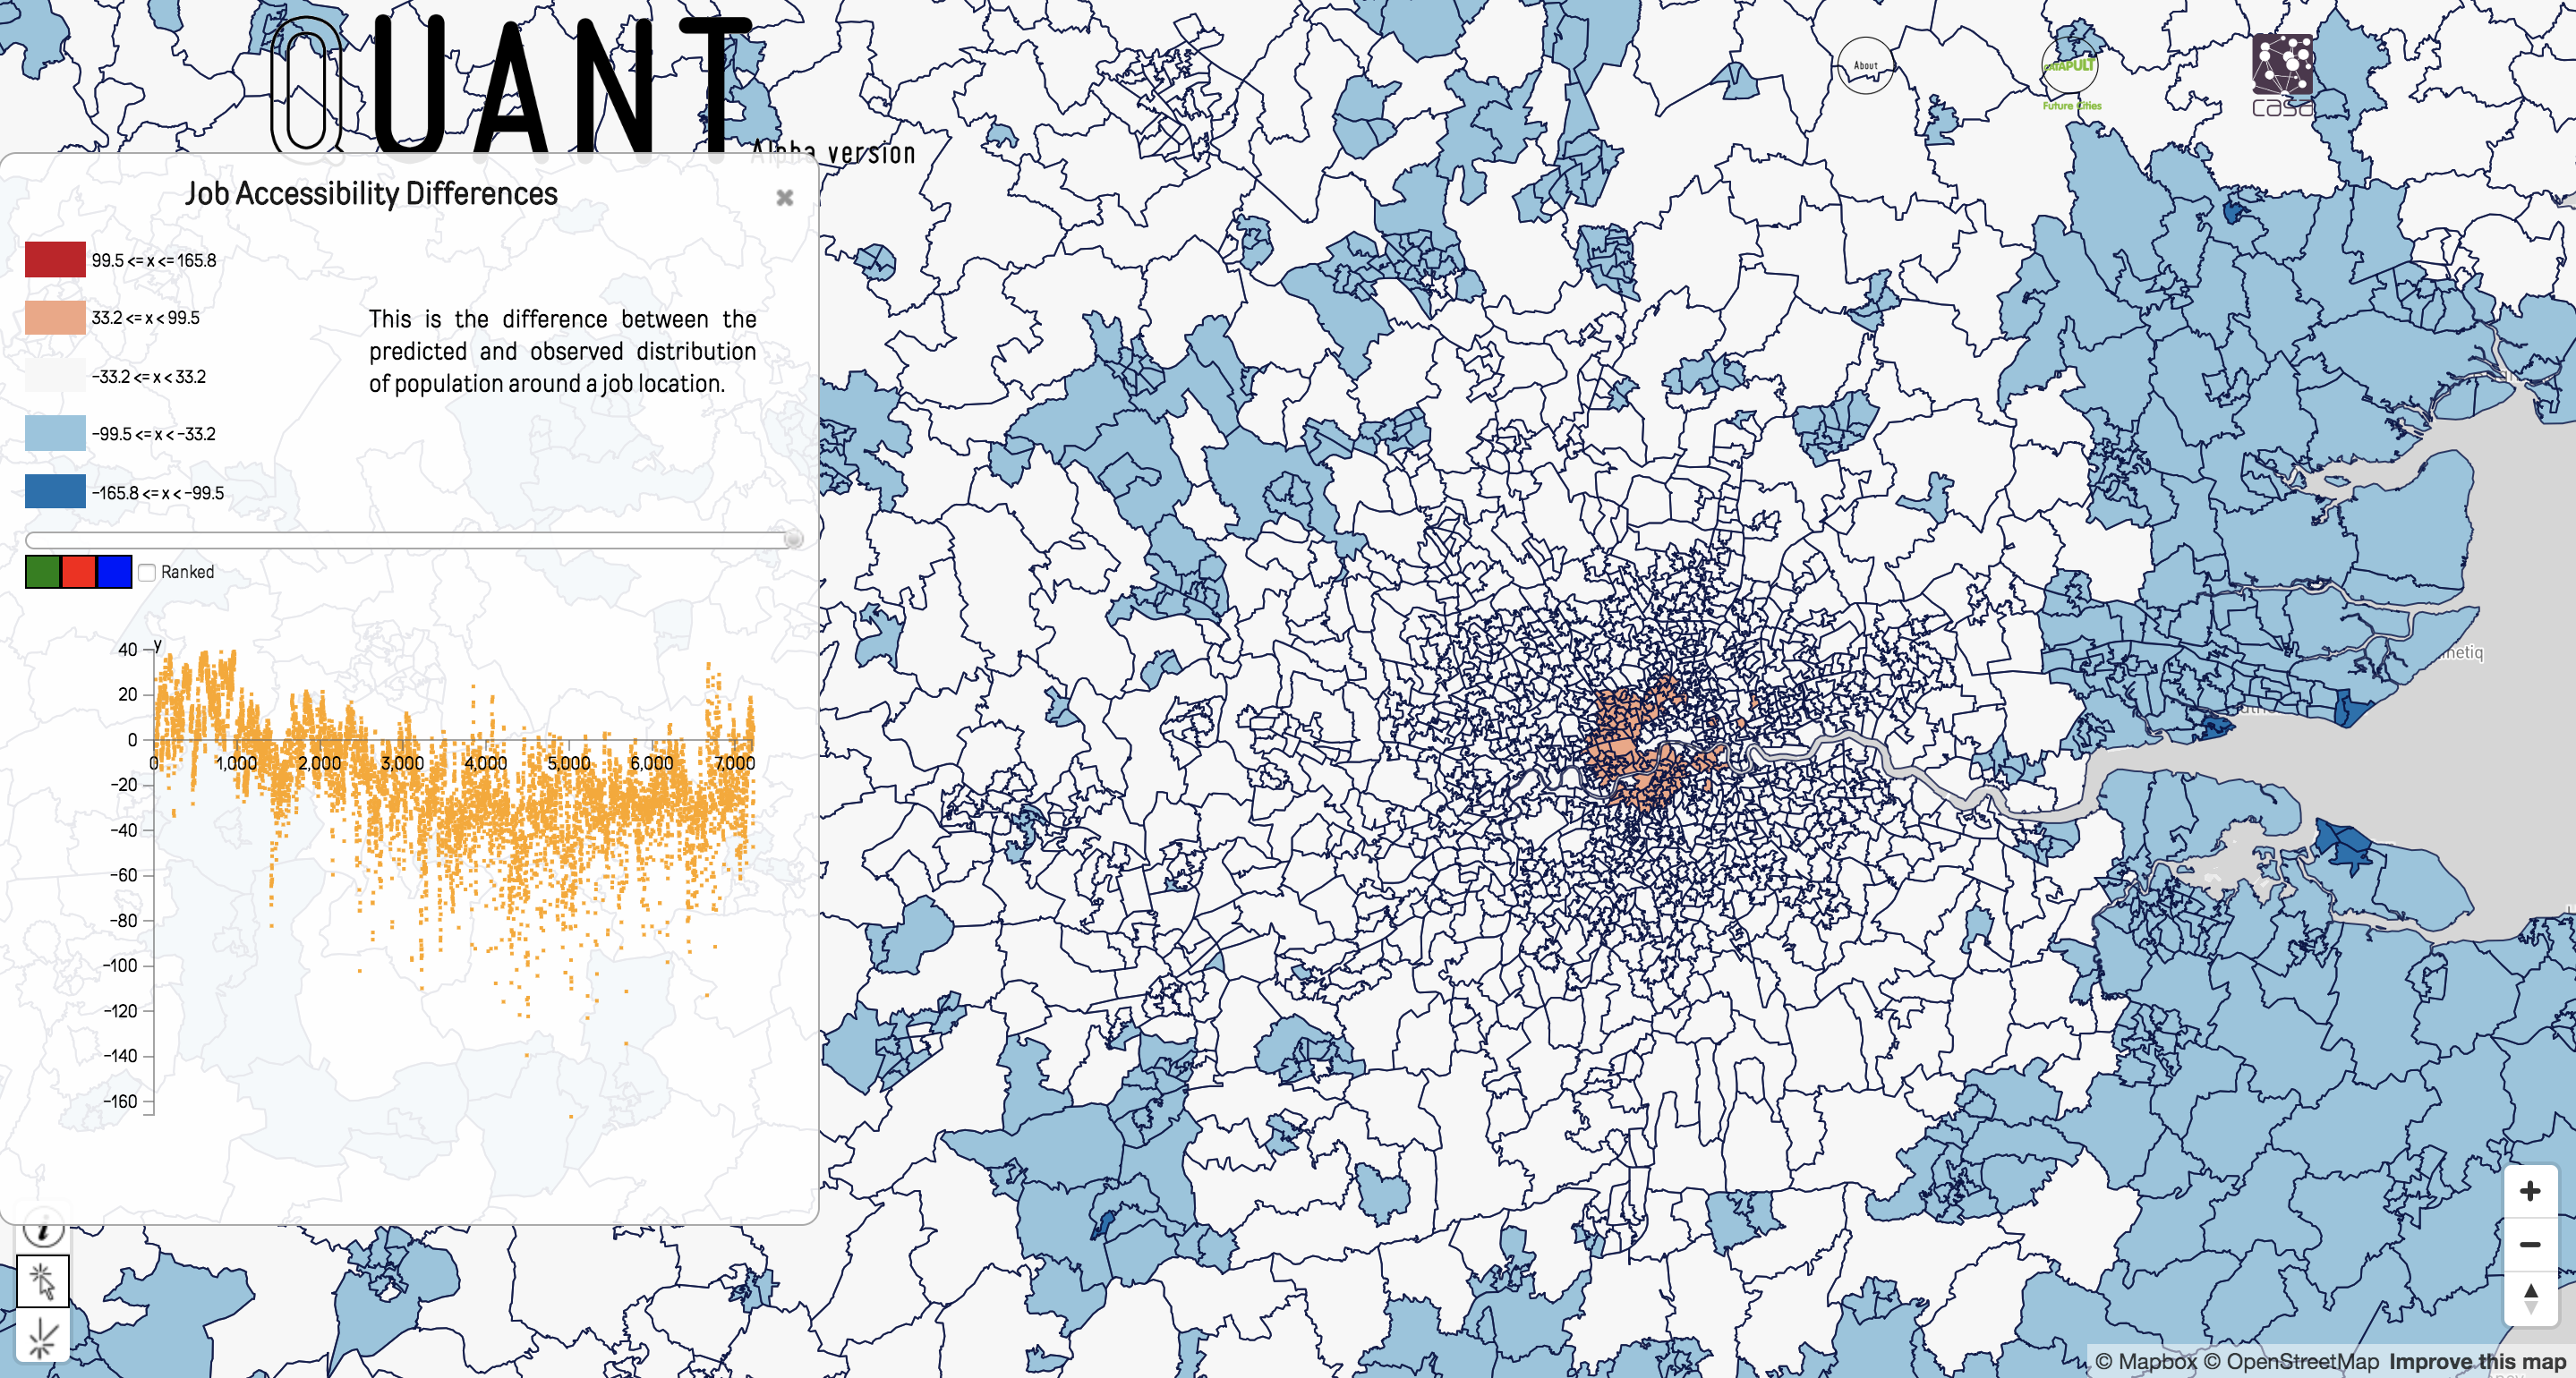
\includegraphics[width=\textwidth]{figures/quant.png}
\end{center}

\medskip

QUANT land-use transport model for Great Britain developed at CASA (PI Michael Batty, Urban Dynamics Lab EPSRC project)

}

\sframe{Coupling Microsimulation and LUTI models}{

\begin{center}
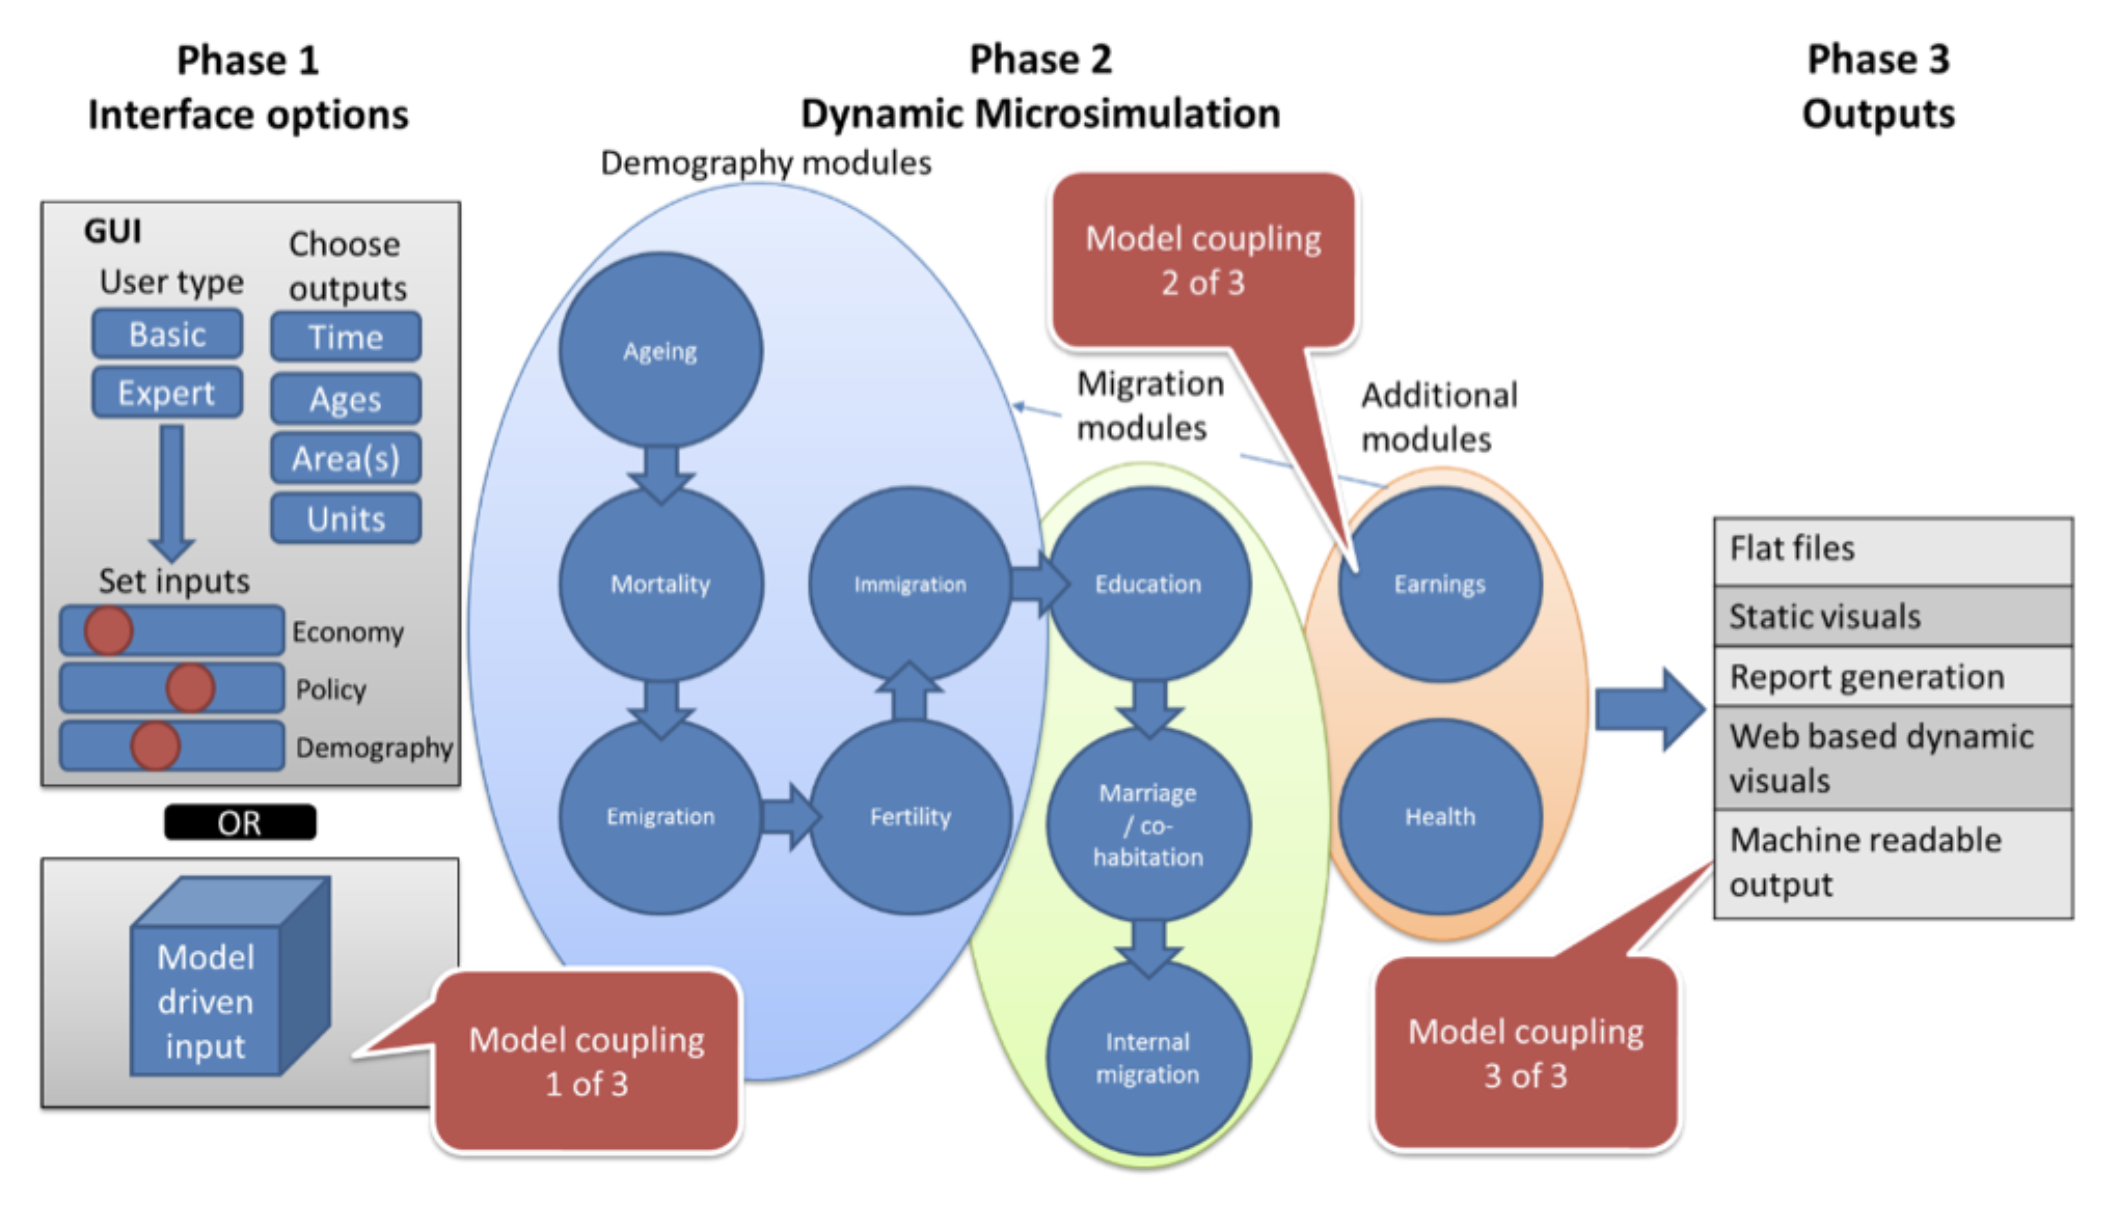
\includegraphics[width=0.95\textwidth]{figures/spenser.png}
\end{center}

\medskip

SPENSER population microsimulation model (population synthesis and projection) developed at University of Leeds (PI Nik Lomaks, ATI project)

}


\sframe{Spatial sensitivity analysis}{

scala library for spatial sensitivity analysis

\texttt{github.com/openmole/spatialdata}

\begin{center}
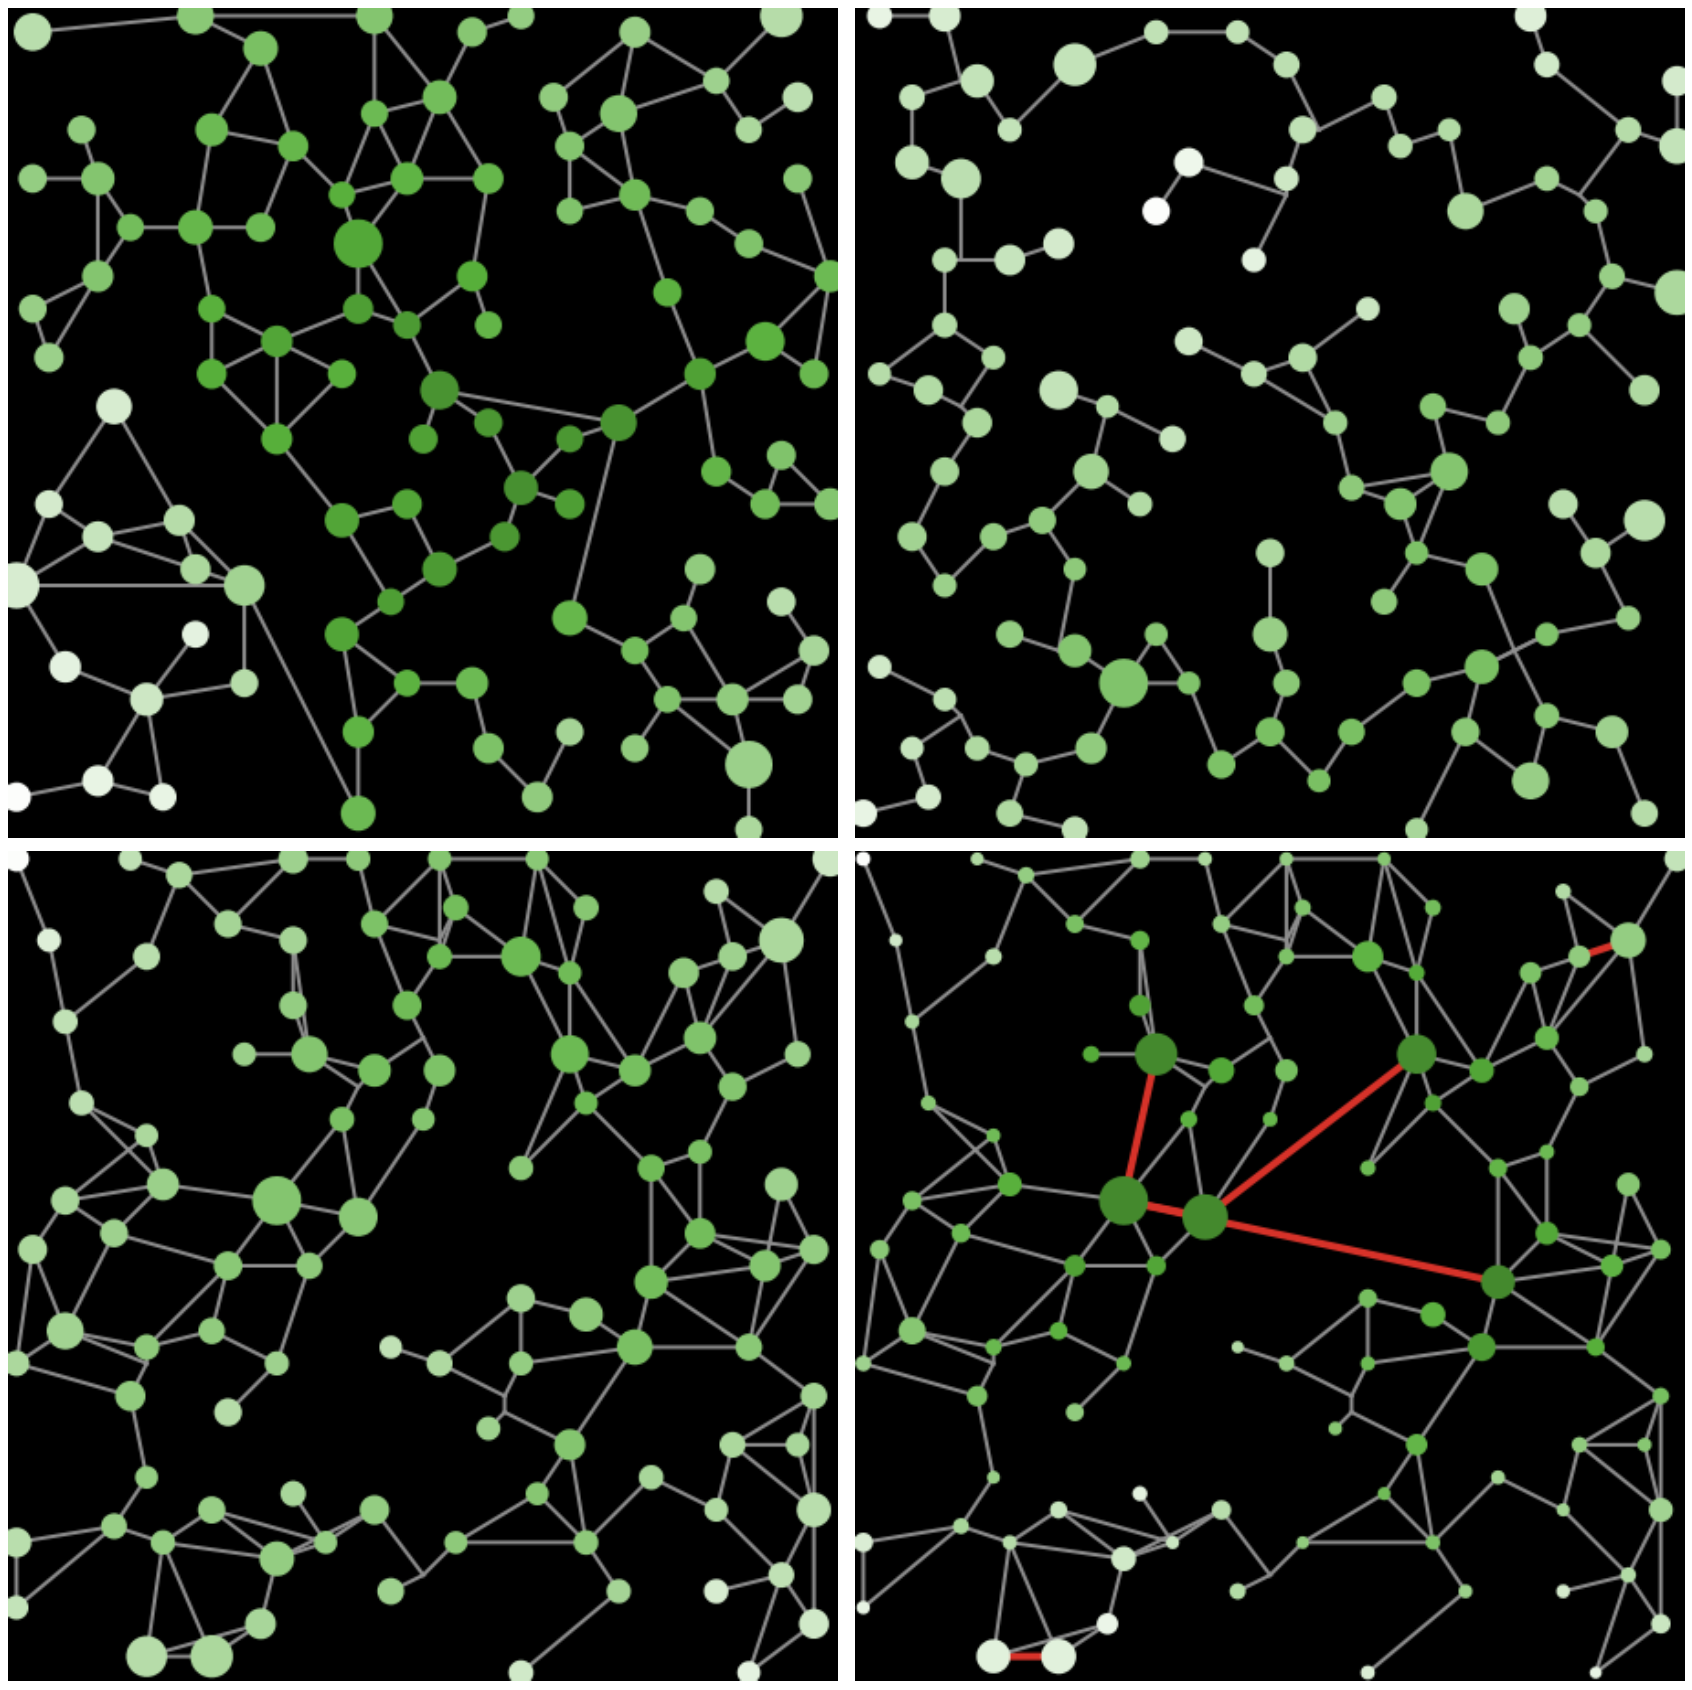
\includegraphics[width=0.42\textwidth]{figures/simpopnet_Fig1.png}
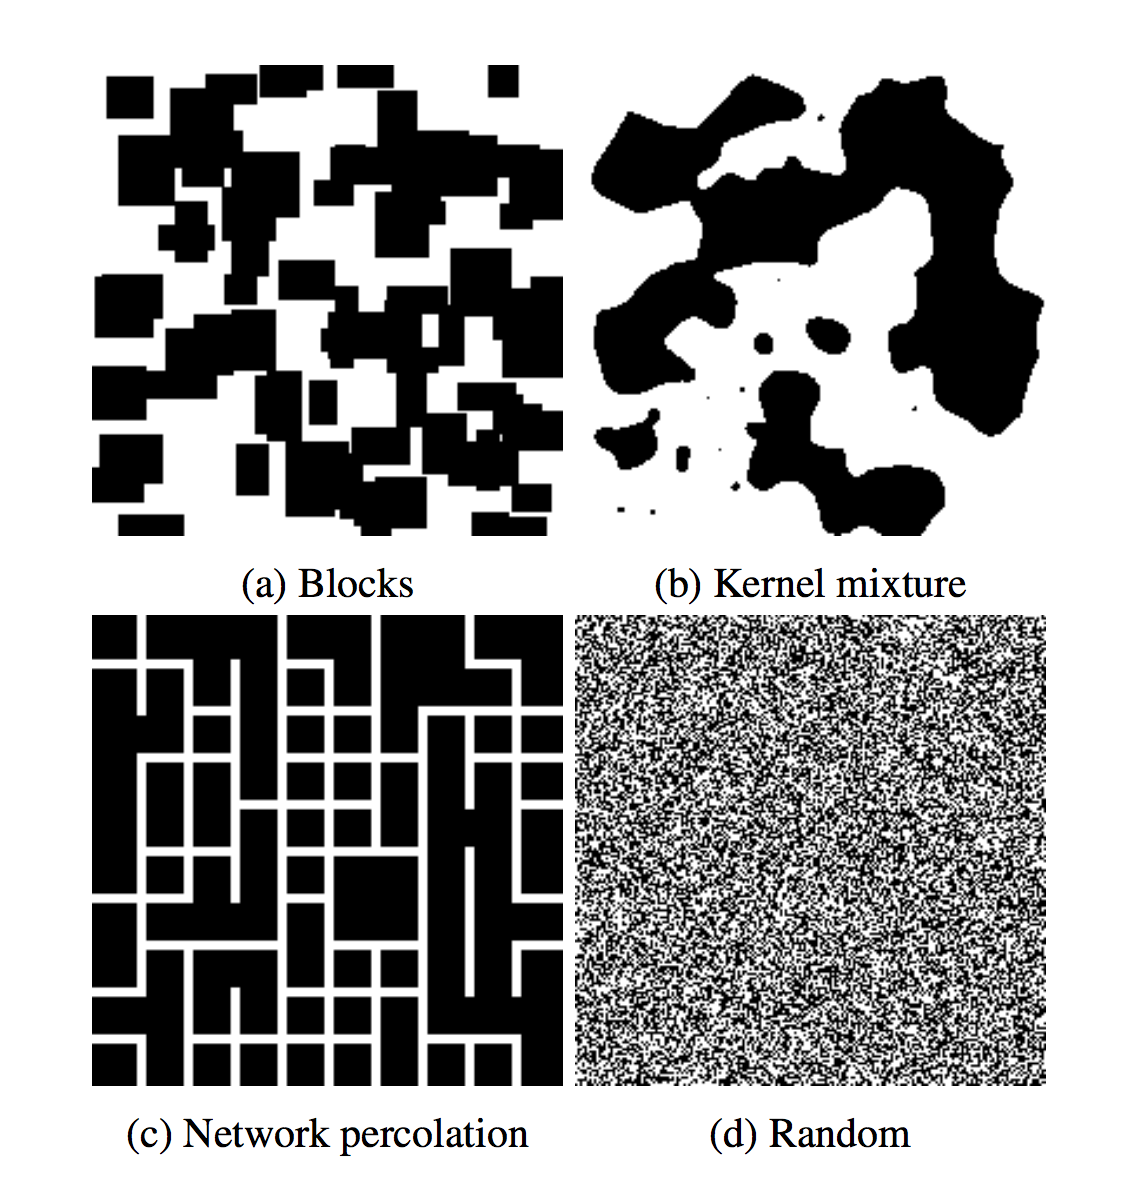
\includegraphics[width=0.42\textwidth]{figures/spatialsens_examplegenerators.png}
\end{center}

\footnotesize

Raimbault, J., Cottineau, C., Le Texier, M., Le Néchet, F., \& Reuillon, R. (2019). Space Matters: Extending Sensitivity Analysis to Initial Spatial Conditions in Geosimulation Models. Journal of Artificial Societies \& Social Simulation, 22(4).

}


\sframe{OpenMOLE integration}{

\textit{Heterogeneity of models and implementations}

\medskip

$\rightarrow$ integration into the OpenMOLE model exploration open source software \texttt{next.openmole.org}
%\cite{reuillon2013openmole}

\begin{center}

\includegraphics[height=0.13\textheight]{figures/iconOM.png}

\includegraphics[height=0.13\textheight]{figures/openmole.png}
\end{center}

\textit{Enables seamlessly (i) model embedding; (ii) access to HPC resources; (iii) exploration and optimization algorithms}

}

\sframe{Expectations}{

\begin{itemize}
	\item Discuss a scala implementation of fast statistical algorithms for population synthesis (IPF, QRIS) and simulation (matrices updates)
	\item Discuss OpenMOLE integration of microsimulation models
	\item Discuss spatial sensitivity analysis in the context of microsimulation
\end{itemize}



}





%%%%%%%%%%%%%%%%%%%%%
%\begin{frame}[allowframebreaks]
%\frametitle{References}
%\bibliographystyle{apalike}
%\bibliography{biblio}
%\end{frame}
%%%%%%%%%%%%%%%%%%%%%%%%%%%%










\end{document}

